%! TeX program = lualatex
\documentclass[12pt,a4paper]{article}

\usepackage[nil]{babel}
\usepackage{unicode-math}
\usepackage[svgnames]{xcolor}
\usepackage{lmodern}
\usepackage{graphicx}
\usepackage{wrapfig}
\usepackage{float}
\usepackage{parskip}
\usepackage[font=small,labelfont=bf]{caption}
\setlength{\emergencystretch}{3em}

\babelprovide[import=el, main, onchar=ids fonts]{greek} % can also do import=el-polyton
\babelprovide[import, onchar=ids fonts]{english}

\babelfont{rm}
          [Language=Default]{Liberation Sans}
\babelfont[english]{rm}
          [Language=Default]{Liberation Sans}
\babelfont{sf}
          [Language=Default]{Liberation Sans}
\babelfont{tt}
          [Language=Default]{Liberation Sans}

%Enter Title Here
 \title{Project-description-v0.2 \\ LibShare}
\author{\textbf{Ονόματα / ΑΜ / Έτος:} \\ Γρηγόρης Καπαδούκας / 1072484 / 4\textdegree \\ Χρήστος Μπεστητζάνος / 1072615 / 4\textdegree \\ Νικόλαος Αυγέρης / 1067508 / 5\textdegree \\ Περικλής Κοροντζής / 1072563 / 4\textdegree}

\begin{document}

\makeatletter
\begin{center}
	\LARGE{\@title} \\
	\pagebreak
	\begin{LARGE}\@author\end{LARGE} \\
\end{center}
\pagebreak

%Insert Body Here
\section{Περιγραφή:}
\label{Περιγραφή}
Το προς δημιουργία project λογισμικού αποτελεί μια εφαρμογή Peer-2-Peer ενοικίασης βιβλίων. Δηλαδή η εφαρμογή αυτή επιτρέπει χρήστες να νοικιάζουν βιβλία ο ένας από τον άλλο για χρηματική ανταμοιβή, με ενσωματωμένη ασφάλεια έναντι κλοπών. Ο χρήστης σε πρώτο βήμα θα μπορεί να δημιουργεί προσωπικό λογαριασμό στην εφαρμογή, εισάγοντας το προσωπικό του email, ένα username και ένα password. Μετά τη δημιουργία του λογαριασμού του ο χρήστης θα μπορεί να εισέρχεται στην εφαρμογή εισάγοντας τα στοιχεία του. Στην εφαρμογή του δίνονται οι εξής δυνατότητες:

\subsection{Σύστημα ενοικιάσεων βιβλίων}
Θα μπορεί να νοικιάσει ένα βιβλίο από άλλους χρήστες της εφαρμογής. Κατά τη λειτουργία αυτή θα του εμφανίζεται μια λίστα από διαθέσιμα βιβλία προς ενοικίαση από άλλους χρήστες της εφαρμογής. Θα υπάρχει δυνατότητα για συναλλαγή πρόσωπο με πρόσωπο, αν οι δύο χρήστες μένουν κοντά και μέσω ταχυδρομικής αποστολής, ασχέτως αν οι χρήστες μένουν κοντά ή μακριά.

Έτσι αφού ο χρήστης κάνει αναζήτηση στη πλατφόρμα και βρει το βιβλίο που θέλει, θα του εμφανίζεται η λίστα των χρηστών που προσφέρουν το βιβλίο αυτό για ενοικίαση. Σε αυτή τη λίστα βλέπει ο χρήστης τους τρόπους συναλλαγής που δέχεται κάθε χρήστης (ταχυδρομικώς ή πρόσωπο με πρόσωπο), την τιμή που ζητάει ο καθένας και το προσωπικό του "σκορ" που προκύπτει από reviews των άλλων χρηστών (θα εξηγηθεί περισσότερο παρακάτω). Αφού επιλέξει έναν μπορεί να του κάνει "Αίτηση ενοικίασης". Έπειτα της αίτησης, ενημερώνεται ο χρήστης - ιδιοκτήτης του βιβλίου και έχει την επιλογή να δεχτεί ή να απορρίψει την αίτηση αυτή.

Αν τη δεχτεί, οι δύο χρήστες βλέπουν τα στοιχεία επικοινωνίας ο ένας του άλλου και αφού λάβει ο ενοικιαστής το βιβλίο ενημερώνουν οι χρήστες την εφαρμογή και χρεώνεται αυτομάτως ο ενοικιαστής ημερήσια, μέχρι το βιβλίο να επιστραφεί στον ιδιοκτήτη και να δηλωθεί η επιστροφή στη πλατφόρμα. 
Αλλιώς αν η αίτηση του ενοικιαστή απορριφθεί, τότε o χρήστης - ενοικιαστής ενημερώνεται και δεν γίνεται συναλλαγή.

Επίσης ο κάθε χρήστης θα μπορεί να αναρτήσει τα βιβλία του στη πλατφόρμα, προσφέροντας τη δυνατότητα στους άλλου χρήστες να νοικιάζουν τα βιβλία του, με χρηματική ανταμοιβή που ορίζει ο ίδιος. Ο χρήστης θα μπορεί επίσης να επεξεργάζεται τη λίστα των βιβλίων που του ανήκουν και προσφέρει για ενοικίαση, προσθέτοντας και αφαιρώντας τυχόν βιβλία.

Ακόμα θα υπάρχει δυνατότητα για τους χρήστες να προβάλλουν το ιστορικό των συναλλαγών τους, μαζί με την κατάσταση των εκκρεμών συναλλαγών και αιτήσεων.

Τέλος οι χρήστες θα μπορούν επίσης έπειτα από μια συναλλαγή να κάνουν reviews ο ένας στον άλλο με τη μορφή 1 έως 5 αστεριών, με προαιρετική προσθήκη σχολίου. Έτσι το συνολικό "σκορ" του κάθε χρήστη εμφανίζεται δίπλα στο όνομά του στη λίστα αναζήτησης βιβλίων και στο προφίλ του φαίνεται το σκορ μαζί με τα σχόλια στους υπόλοιπους χρήστες.

\subsection{Αναζήτηση άλλων χρηστών, προσθήκη αγαπημένων χρηστών και σύστημα ενημερώσεων}
Ο χρήστης θα μπορεί επίσης να κάνει αναζήτηση άλλου χρήστη με βάση το username τους και να δει τα στοιχεία τους (username, το σκορ και τα σχόλιά του, την πόλη που μένει, ένα description που ορίζει ο ίδιος) και τα βιβλία που προσφέρει για ενοικίαση.

Επίσης θα υπάρχει δυνατότητα για προσθήκη των άλλων χρηστών στη λίστα "Αγαπημένων", όπου τα βιβλία που τους ανήκουν και προσφέρονται για ενοικίαση εμφανίζονται με προτεραιότητα στη λίστα των διαθέσιμων βιβλίων κατά την αναζήτηση.

Επίσης το σύστημα των αγαπημένων θα συνδέεται με το σύστημα των ενημερώσεων, με το οποίο ο χρήστης ενημερώνεται από το σύστημα όταν ένας χρήστης στη λίστα αγαπημένων του προσθέτει νέο βιβλίο προς ενοικίαση στο σύστημα.

\subsection{Σύστημα αιτήσεων βιβλίων που δεν προσφέρονται ήδη στην πλατφόρμα}
Θα υπάρχει επίσης λειτουργικότητα για τους χρήστες να δημιουργούν και να προβάλλουν "αιτήματα" για βιβλία που δεν υπάρχουν διαθέσιμα προς ενοικίαση στην πλατφόρμα, με προσφορά επιπλέον ανταμοιβής σε όποιον ιδιοκτήτη του βιβλίου αυτού το προσφέρει στον χρήστη που το ζητάει. Με αυτόν τον τρόπο διευκολύνεται η εύρεση βιβλίων που δεν είναι ήδη διαθέσιμα στη πλατφόρμα.

Επίσης θα μπορεί ο χρήστης να αναζητεί, να προβάλλει και να πληρεί αιτήσεις άλλων χρηστών, εφόσον έχει το βιβλίο που ζητείται, και έτσι να κάνει αίτηση εκπλήρωσης αίτησης στον χρήστη που την έφτιαξε και να αρχικοποιηθεί συναλλαγή μαζί του.

\subsection{Σύστημα διαχείρισης λογαριασμών}
Ο χρήστης θα μπορεί να προβάλλει και να αλλάζει τα στοιχεία του, δηλαδή το username, το email το, σύντομο description, τη πόλη κατοικίας, την  εικόνα χρήστη και τον κωδικό πρόσβασής του. Θα μπορεί επίσης να προσθέσει και να αφαιρέσει λεφτά από τον λογαριασμό του. 

\subsection{Σύστημα προστασίας χρηστών από κλοπές και φθορές}
Για την προστασία των ιδιοκτητών από κλοπές, θα γίνεται αυτόματη μεταφορά των χρημάτων μεταξύ χρηστών κατά τη διάρκεια μιας ενοικίαση. 

Επίσης για να επιτευχθεί μια ενοικίαση δεσμεύεται ένα "ποσό ασφαλείας" από τον ενοικιαστή, με σκοπό την προστασία του ιδιοκτήτη από κλοπή ή φθορά του βιβλίου. Στην περίπτωση που η συναλλαγή ολοκληρωθεί χωρίς κανένα θέμα το ποσό αυτό ασφαλείας θα επιστρέφεται στον ενοικιαστή αυτομάτως.

Στην περίπτωση όμως διαμάχης μεταξύ ενοικιαστή και ιδιόκτητη θα υπάρχει δυνατότητα επικοινωνίας με υποστήριξη πελατών με σκοπό την επίλυση των διαφωνιών όπου είναι εφικτό. Παραδείγματα διαμαχών μπορεί να είναι η κλοπή ή φθορά του βιβλίου, όπου ο ιδιοκτήτης αποζημιώνεται μέσω του "ποσού ασφαλείας" ή θα μπορούσε να είναι η αποστολή ταχυδρομικώς του λάθους βιβλίου, όπου ο ενοικιαστής δεν χρειάζεται να πληρώσει τίποτα, και του αποδεσμεύεται αμέσως το "ποσό ασφαλείας". Και στις δύο περιπτώσεις το άτομο με κακή τιμωρείται από την πλατφόρμα με περιορισμούς στις ενοικιάσεις, και από τους ίδιους τους χρήστες μέσω των κακών σκορ.

Η υποστήριξη πελατών σημειώνουμε λειτουργεί με βάση προκαθορισμένης πολιτικής προστασίας πελατών. Έχει σκοπό να τιμωρήσει κακόβουλες συμπεριφορές και έχει τη δυνατότητα να αποδεσμεύσει το ποσό προκαταβολής και να το χρησιμοποιήσει για να αποζημιωθούν οι χρήστες, μόνο όταν το ορίζει η πολιτική.

\section{Mock-up Οθόνες}

\textbf{Σημέιωση:} Οι οθόνες στο κεφάλαιο αυτό είναι ενδεικτικές και δεν θα αποτελούν αναγκαστικά την ακριβή δομή του τελικού project. Λειτουργούν παραπάνω για ένδειξη του περιεχομένου της τελικής οθόνης και όροι όπως "στο κάτω μέρος της οθόνης" αναφέρονται μόνο στη δομή του σχήματος που δίνεται και όχι αναγκαστικά του τελικού project.

\subsection{Search}

Για την οθόνη της αναζήτησης έχουμε ορίσει τρεις περιπτώσεις (με βάση τα φίλτρα που εισάγει ο χρήστης), οι οποίες αποτελούν τα σχήματα \ref{Οθόνη "Search Book" λειτουργικότητας},

\subsubsection{Search Book}

Στο Σχήμα \ref{Οθόνη "Search Book" λειτουργικότητας} παρουσιάζεται mock-up οθόνη της λειτουργικότητας της αναζήτησης βιβλίων και της δημιουργίας αίτησης ενοικίασης.

\begin{figure}[H]
	\makebox[\textwidth]{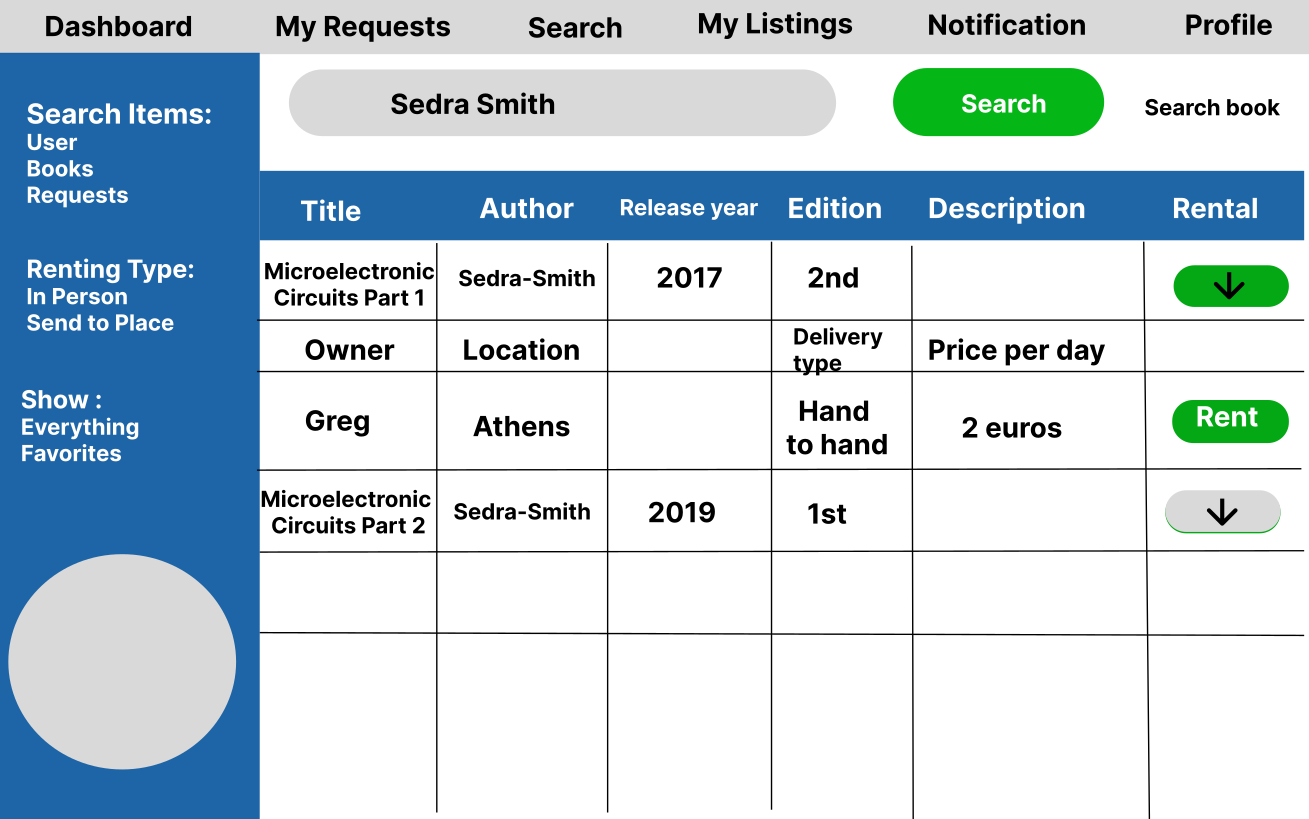
\includegraphics[width=\textwidth]{Mockup Screens/Search Book.png}}
	\caption{Οθόνη "Search Book" λειτουργικότητας}
	\label{Οθόνη "Search Book" λειτουργικότητας}
\end{figure}

Ο χρήστης δίπλα σε κάθε βιβλίο έχει τη δυνατότητα να πατήσει το drop down μενού, οπότε μετά του εμφανίζονται οι ιδιοκτήτες που έχουν διαθέσιμο το βιβλίο προς ενοικίαση.

Η λειτουργικότητα του "Rent" είναι αυτή που εξηγείται ως "αίτηση ενοικίασης" στο κεφάλαιο \ref{Περιγραφή}.

\subsubsection{Search User}

Στο Σχήμα \ref{Οθόνη "Search User" λειτουργικότητας} παρουσιάζεται mock-up οθόνη της λειτουργικότητας της αναζήτησης χρηστών.

\begin{figure}[H]
	\makebox[\textwidth]{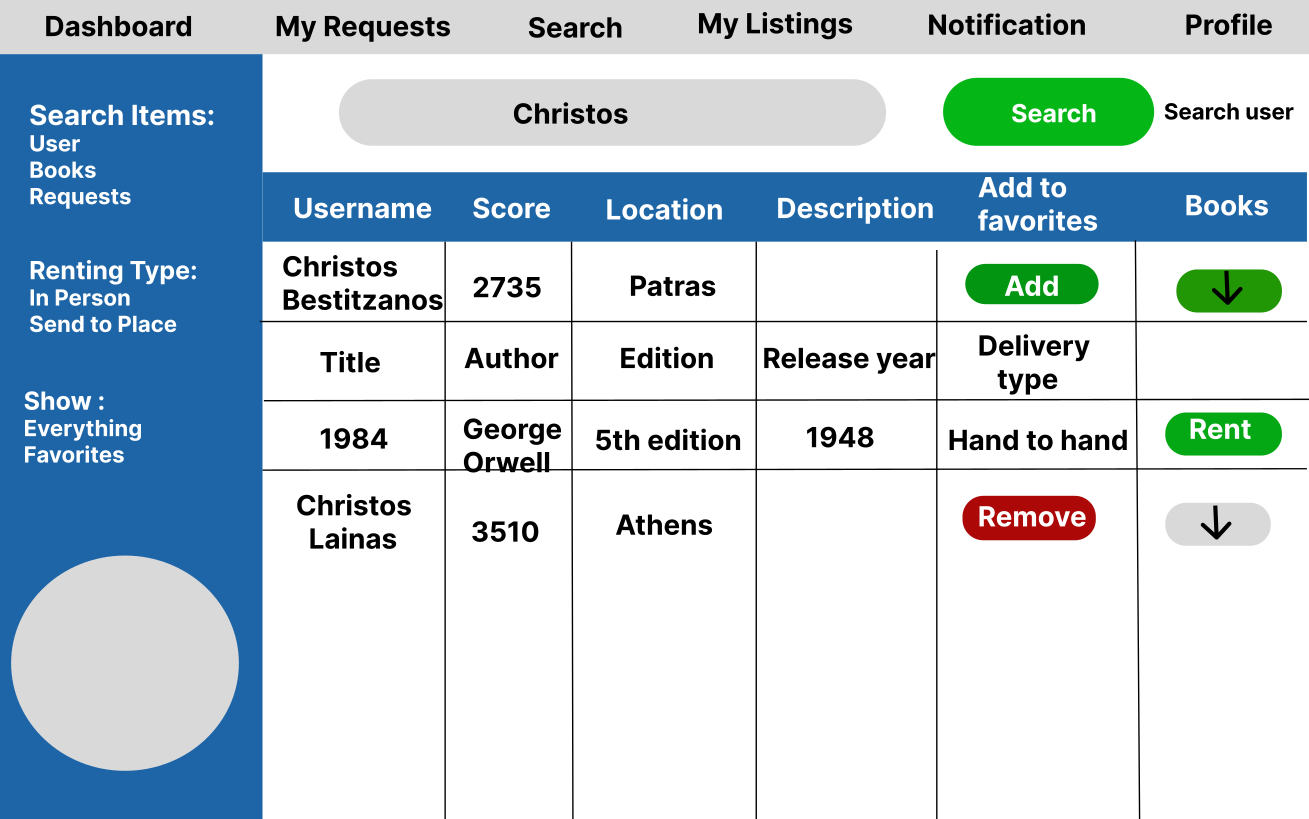
\includegraphics[width=\textwidth]{Mockup Screens/Search User.png}}
	\caption{Οθόνη "Search User" λειτουργικότητας}
	\label{Οθόνη "Search User" λειτουργικότητας}
\end{figure}

Ο χρήστης έχει επίσης έχει τη δυνατότητα να τον προσθέσει στη λίστα των αγαπημένων του, καθώς και να προβάλλει τα διαθέσιμα βιβλία που έχει προς ενοικίαση, μέσω του drop down μενού. 

Πατώντας έπειτα το κουμπί "Rent", γίνεται πάλι αίτηση ενοικίασης.

\subsubsection{Search Requests}

Στο Σχήμα \ref{Οθόνη "Search Requests" λειτουργικότητας} παρουσιάζεται mock-up οθόνη της λειτουργικότητας της αναζήτησης αιτήσεων που έχουν κάνει άλλοι χρήστες.

\begin{figure}[H]
	\makebox[\textwidth]{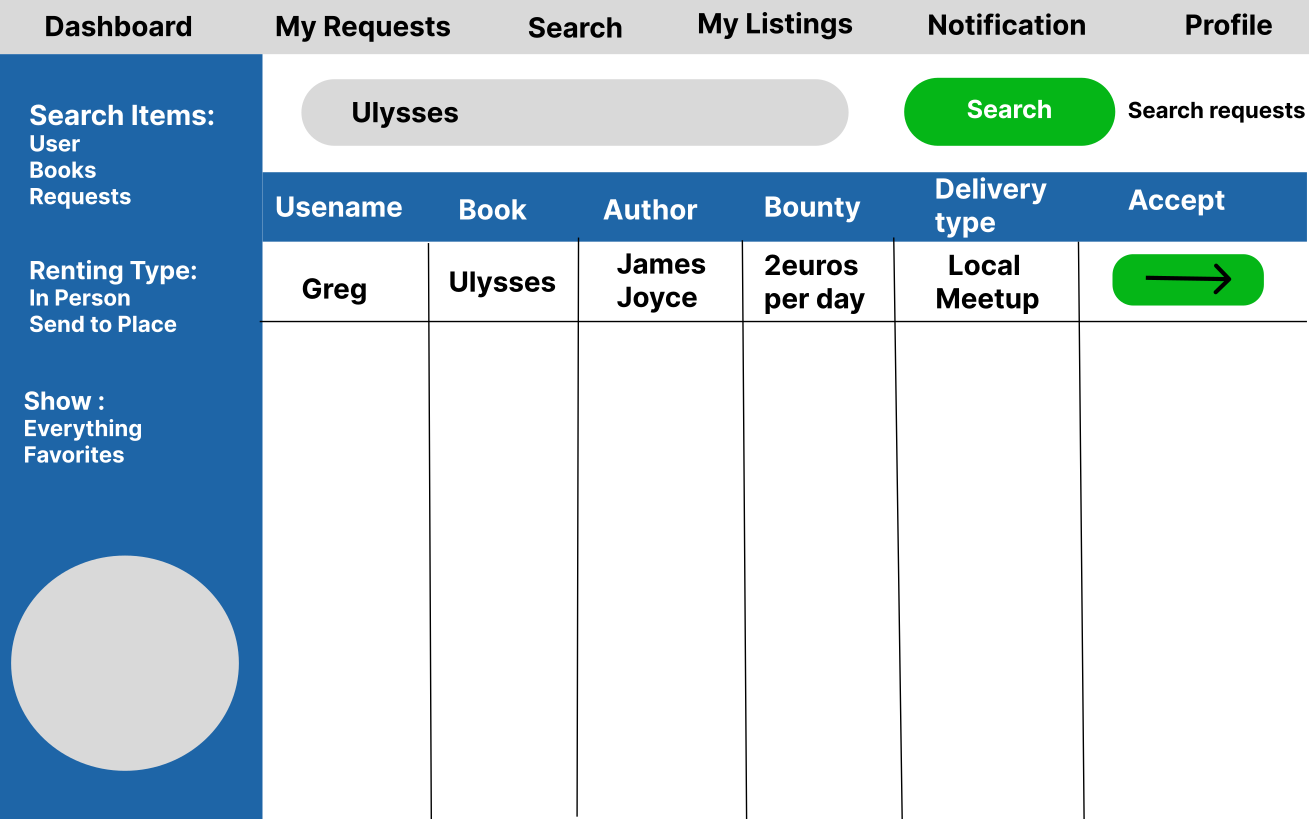
\includegraphics[width=\textwidth]{Mockup Screens/Search Request.png}}
	\caption{Οθόνη "Search Requests" λειτουργικότητας}
	\label{Οθόνη "Search Requests" λειτουργικότητας}
\end{figure}

Ο χρήστης στην οθόνη αυτή μπορεί να προβάλλει και να αναζητεί τις αιτήσεις άλλων χρηστών και έχει τη δυνατότητα να δεχτεί τις αιτήσεις αυτές αν έχει το βιβλίο που ζητείται. Μέσω του κουμπιού "Accept" δημιουργείται μια νέα συναλλαγή με τον χρήστη που αιτεί το βιβλίο.

\subsection{Dashboard}

Στο Σχήμα \ref{Οθόνη "Dashboard" λειτουργικότητας} παρουσιάζεται mock-up οθόνη της οθόνης "Dashboard" που δείχνει τις τρέχουσες συναλλαγές με δυνατότητα χειρισμού του και ανανέωσης της κατάστασης στις οποίες βρίσκονται.

\begin{figure}[H]
	\makebox[\textwidth]{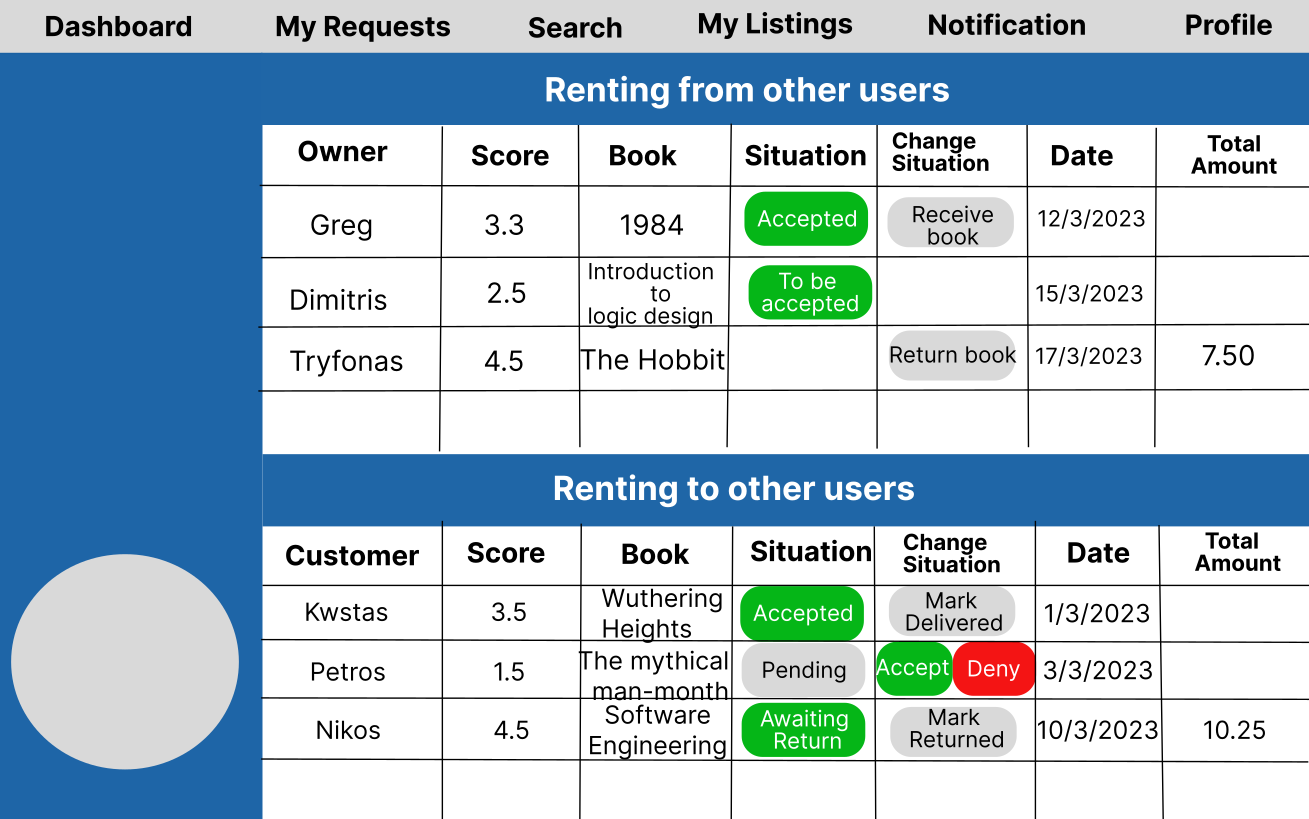
\includegraphics[width=\textwidth]{Mockup Screens/Dashboard.png}}
	\caption{Οθόνη "Dashboard" λειτουργικότητας}
	\label{Οθόνη "Dashboard" λειτουργικότητας}
\end{figure}

Παρατηρούμε ότι στους πίνακες έχουμε το πεδίο "Situation" στο οποίο αναφέρεται η κατάσταση στην οποία βρίσκεται η συναλλαγή (πχ αναμονή για αποδοχή από τον ιδιοκτήτη, αναμονή για επιστροφή κτλ).

Επίσης με το πεδίο "Change Situation" έχουμε παραθέσει τα κουμπιά με τα οποία ο χρήστης αλλάζει τις καταστάσεις (πχ αποδοχή αιτήματος, δήλωση επιστροφής βιβλίου κτλ).

\subsection{My Listings}

Στο Σχήμα \ref{Οθόνη "My Listings" λειτουργικότητας} παρουσιάζεται mock-up οθόνη της λειτουργικότητας της προβολής των βιβλίων που προσφέρει ο χρήστης σε άλλους να νοικιάσουν, μαζί με δυνατότητα προσθήκης και αφαίρεσης άλλων βιβλίων.

\begin{figure}[H]
	\makebox[\textwidth]{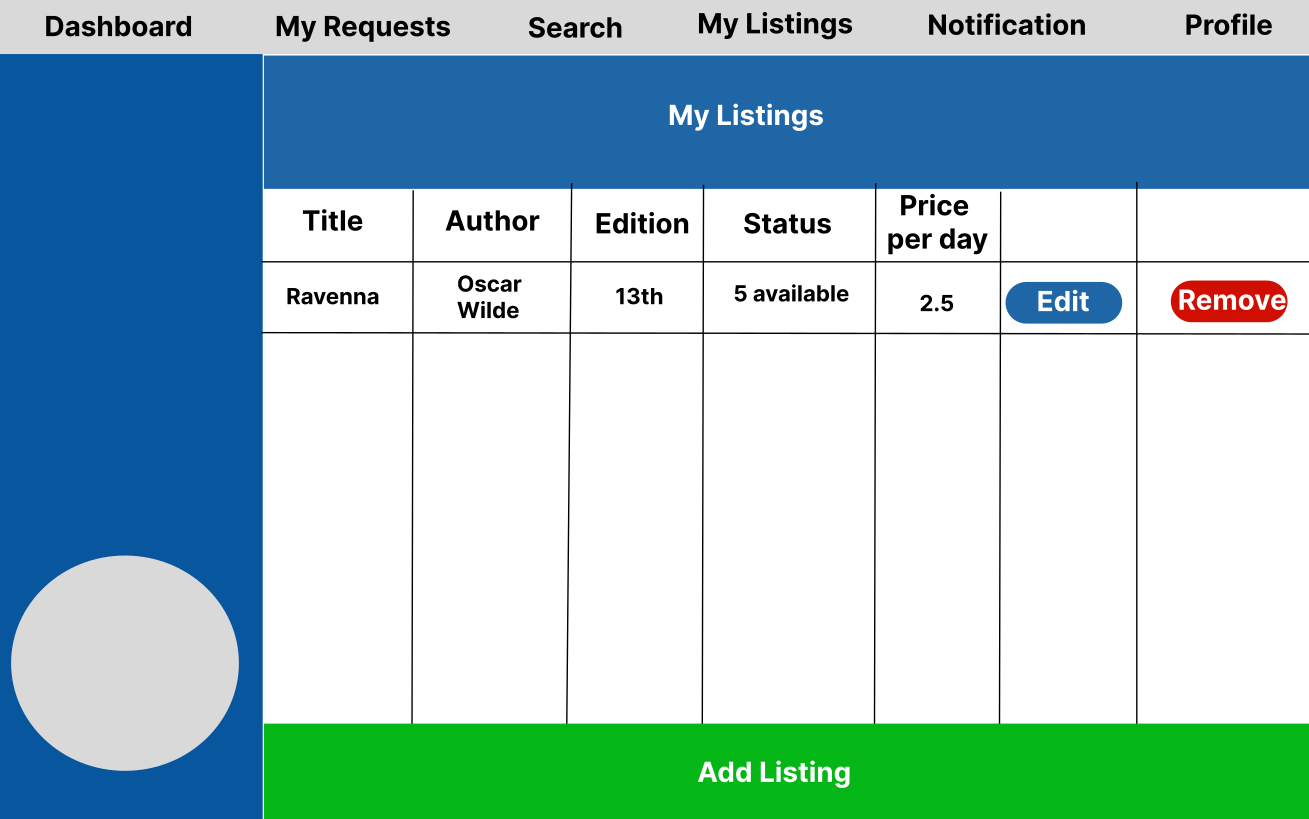
\includegraphics[width=\textwidth]{Mockup Screens/My Listings.png}}
	\caption{Οθόνη "My Listings" λειτουργικότητας}
	\label{Οθόνη "My Listings" λειτουργικότητας}
\end{figure}

Πατώντας το κουμπί "Edit" ή το κουμπί "Add Listing" εμφανίζεται pop up οθόνη στην οποία ο χρήστης αλλάζει ή προσθέτει αντίστοιχα τα στοιχεία του βιβλίου, την τιμή και το τρόπο συναλλαγής. Ένα mock up screen της οθόνης αυτής φαίνεται στο Σχήμα \ref{Οθόνη "Add Book Details" λειτουργικότητας}.

\begin{figure}[H]
	\makebox[\textwidth]{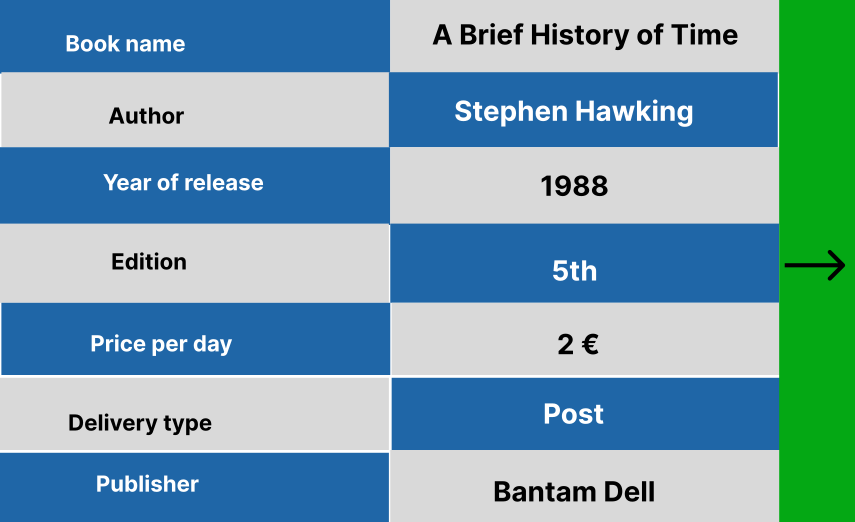
\includegraphics[width=\textwidth]{Mockup Screens/Add Book Details Popup.png}}
	\caption{Οθόνη "Add Book Details" λειτουργικότητας}
	\label{Οθόνη "Add Book Details" λειτουργικότητας}
\end{figure}


\subsection{My Requests}

Στο Σχήμα \ref{Οθόνη "My Requests" λειτουργικότητας} παρουσιάζεται mock-up οθόνη της λειτουργικότητας της προβολή των αιτήσεων που έχει κάνει ο χρήστης, μαζί με δυνατότητα προσθήκης και αφαίρεσής τους.

\begin{figure}[H]
	\makebox[\textwidth]{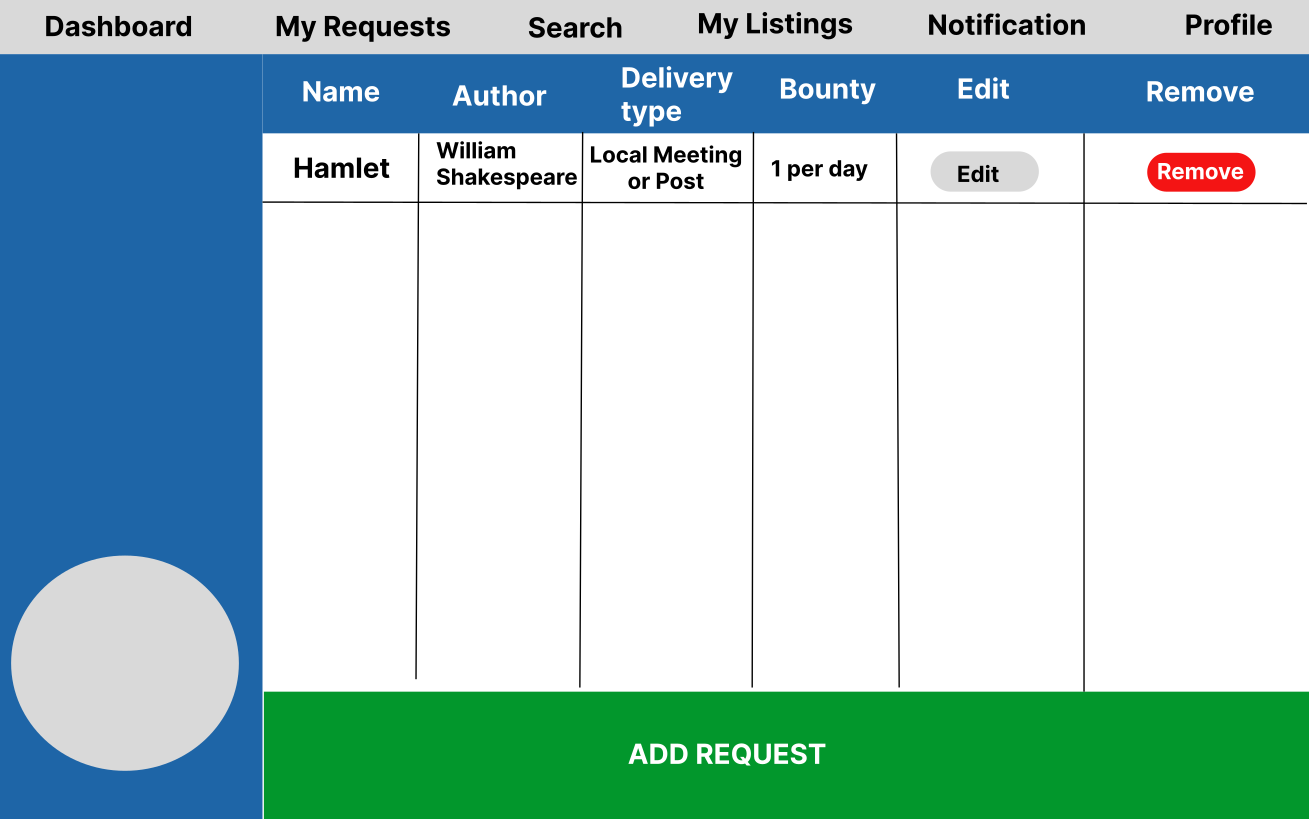
\includegraphics[width=\textwidth]{Mockup Screens/My Requests.png}}
	\caption{Οθόνη "My Requests" λειτουργικότητας}
	\label{Οθόνη "My Requests" λειτουργικότητας}
\end{figure}

Πατώντας το κουμπί "Edit" ή το κουμπί "Add Request" εμφανίζεται pop up οθόνη στην οποία ο χρήστης αλλάζει ή προσθέτει αντίστοιχα τα στοιχεία της αίτησης, η οποία θα μοιάζει πάλι σαν την οθόνη του Σχήματος \ref{Οθόνη "Add Book Details" λειτουργικότητας}.


\subsection{Transaction History}

Στο Σχήμα \ref{Οθόνη "Transaction History" λειτουργικότητας} παρουσιάζεται mock-up οθόνη της λειτουργικότητας της προβολής των τελειωμένων συναλλαγών, μαζί με τη δυνατότητα προβολής στατιστικών και την δυνατότητα επιλογής φίλτρων για την αναζήτηση στο ιστορικό.

\begin{figure}[H]
	\makebox[\textwidth]{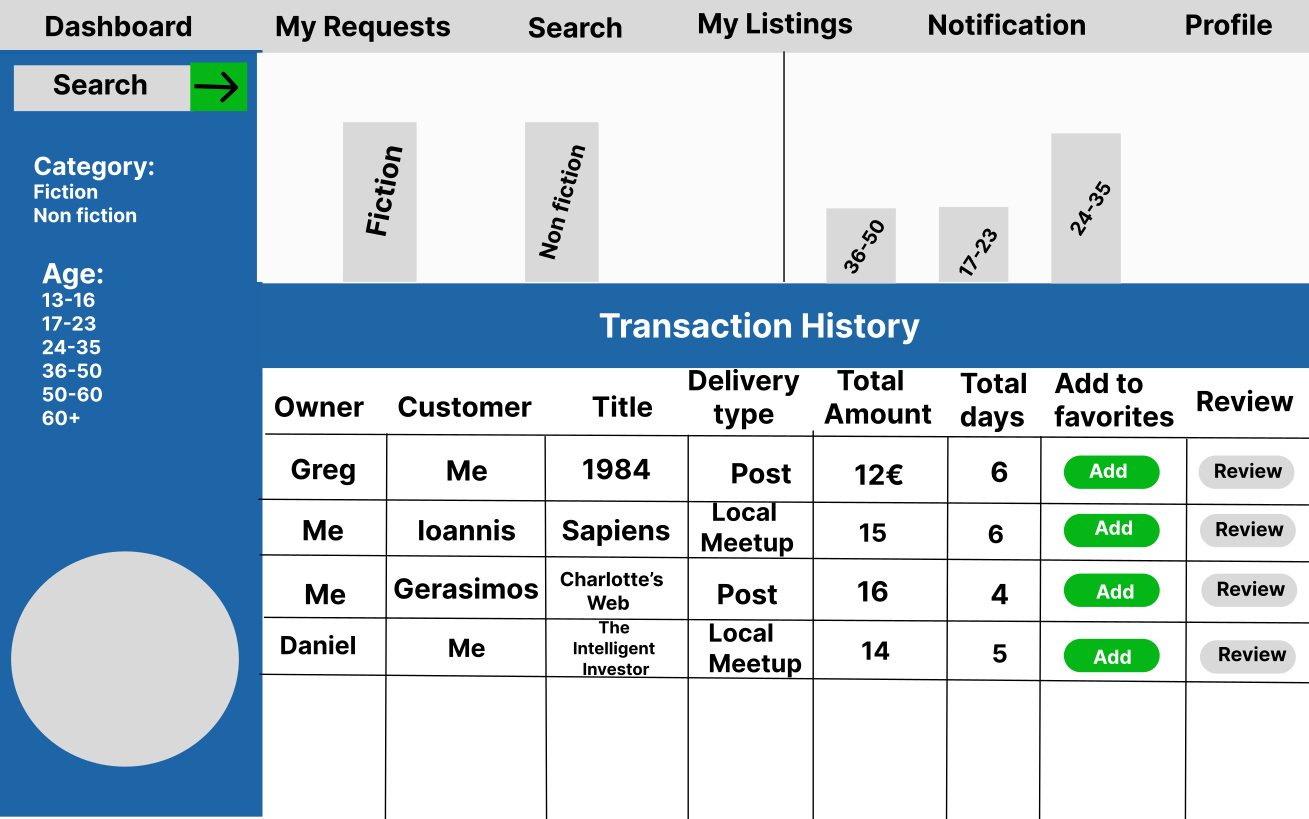
\includegraphics[width=\textwidth]{Mockup Screens/Transaction History.png}}
	\caption{Οθόνη "Transaction History" λειτουργικότητας}
	\label{Οθόνη "Transaction History" λειτουργικότητας}
\end{figure}

Στην οθόνη αυτή υπάρχει επίσης η δυνατότητα για τον χρήστη να προσθέσει τον άλλο χρήστη με τον οποίο έκανε τη συναλλαγή στη λίστα αγαπημένων του, και την καταχώρηση αξιολόγησης για τον χρήστη αυτόν, με τη μορφή ενός έως πέντε "αστεράκια" και προαιρετική εισαγωγή σχολίου.

Στο Σχήμα \ref{Οθόνη "Star Rating" λειτουργικότητας} φαίνεται η δυνατότητα αξιολόγησης με τα "αστεράκια" και στο Σχήμα \ref{Οθόνη "Comment Rating" λειτουργικότητας} φαίνεται η δυνατότητα συγγραφής του προαιρετικού σχολίου.

\begin{figure}[H]
    \makebox[\textwidth]{\fbox{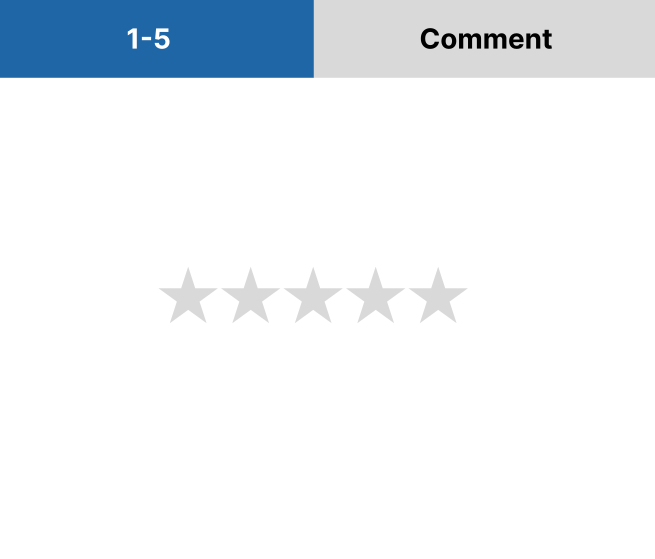
\includegraphics[width=\textwidth]{Mockup Screens/Star Rating.png}}}
	\caption{Οθόνη "Star Rating" λειτουργικότητας}
	\label{Οθόνη "Star Rating" λειτουργικότητας}
\end{figure}

\begin{figure}[H]
    \makebox[\textwidth]{\fbox{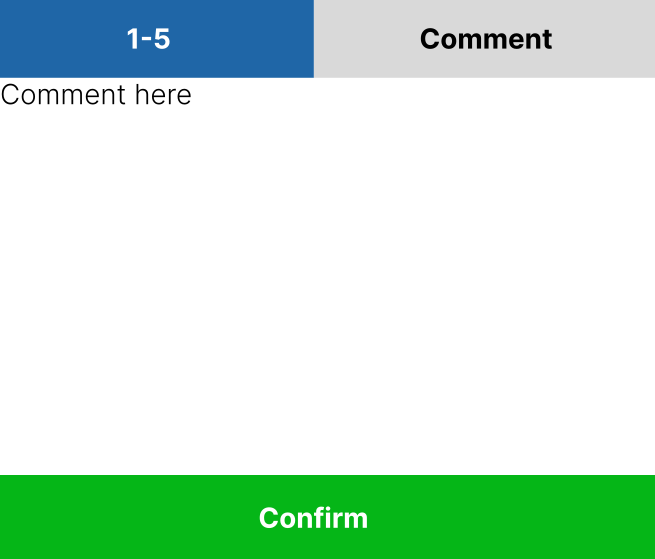
\includegraphics[width=\textwidth]{Mockup Screens/Comment Rating.png}}}
	\caption{Οθόνη "Comment Rating" λειτουργικότητας}
	\label{Οθόνη "Comment Rating" λειτουργικότητας}
\end{figure}

\subsection{Notifications:}

Στο Σχήμα \ref{Οθόνη "Notifications" λειτουργικότητας} παρουσιάζεται mock-up οθόνη της λειτουργικότητας της προβολής ειδοποιήσεων, που δημιουργούνται αυτόματα όταν ένας "αγαπημένος" χρήστης του χρήστη προσθέτει ένα νέο βιβλίο προς ενοικίαση από άλλους ή προσθέτει μια νέα αίτηση.

\begin{figure}[H]
	\makebox[\textwidth]{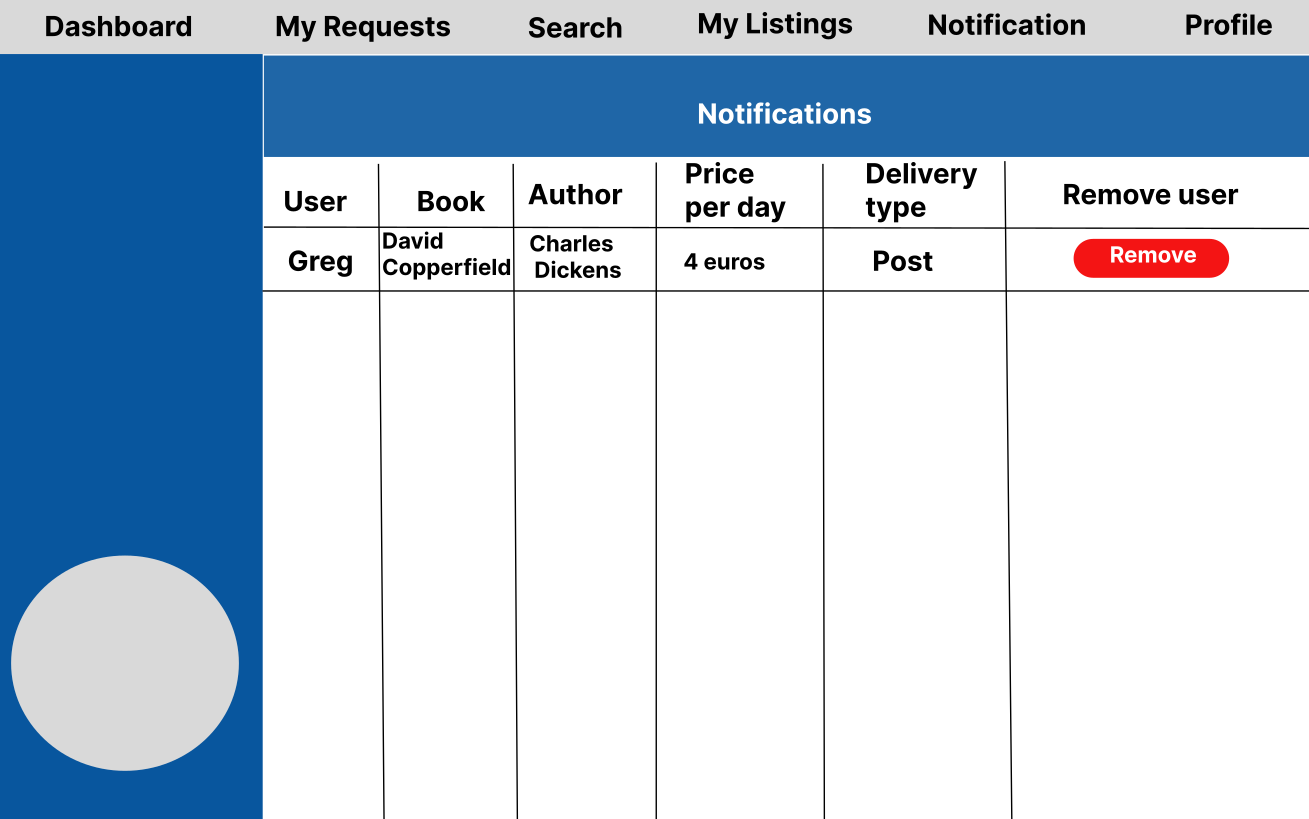
\includegraphics[width=\textwidth]{Mockup Screens/Notifications.png}}
	\caption{Οθόνη "Notifications" λειτουργικότητας}
	\label{Οθόνη "Notifications" λειτουργικότητας}
\end{figure}

Στην οθόνη αυτή υπάρχει ένα κουμπί αφαίρεσης του χρήστη από τη λίστα αγαπημένων, οπότε μετά από αυτό δεν θα εμφανίζονται πλέον ειδοποιήσεις σχετικές με αυτόν τον χρήστη.

\subsection{Profile και Balance}

Στο Σχήμα \ref{Οθόνη "My Profile" λειτουργικότητας} παρουσιάζεται mock-up οθόνη της λειτουργικότητας της προβολής και αλλαγής των στοιχείων του λογαριασμού του συνδεδεμένου χρήστη.

\begin{figure}[H]
	\makebox[\textwidth]{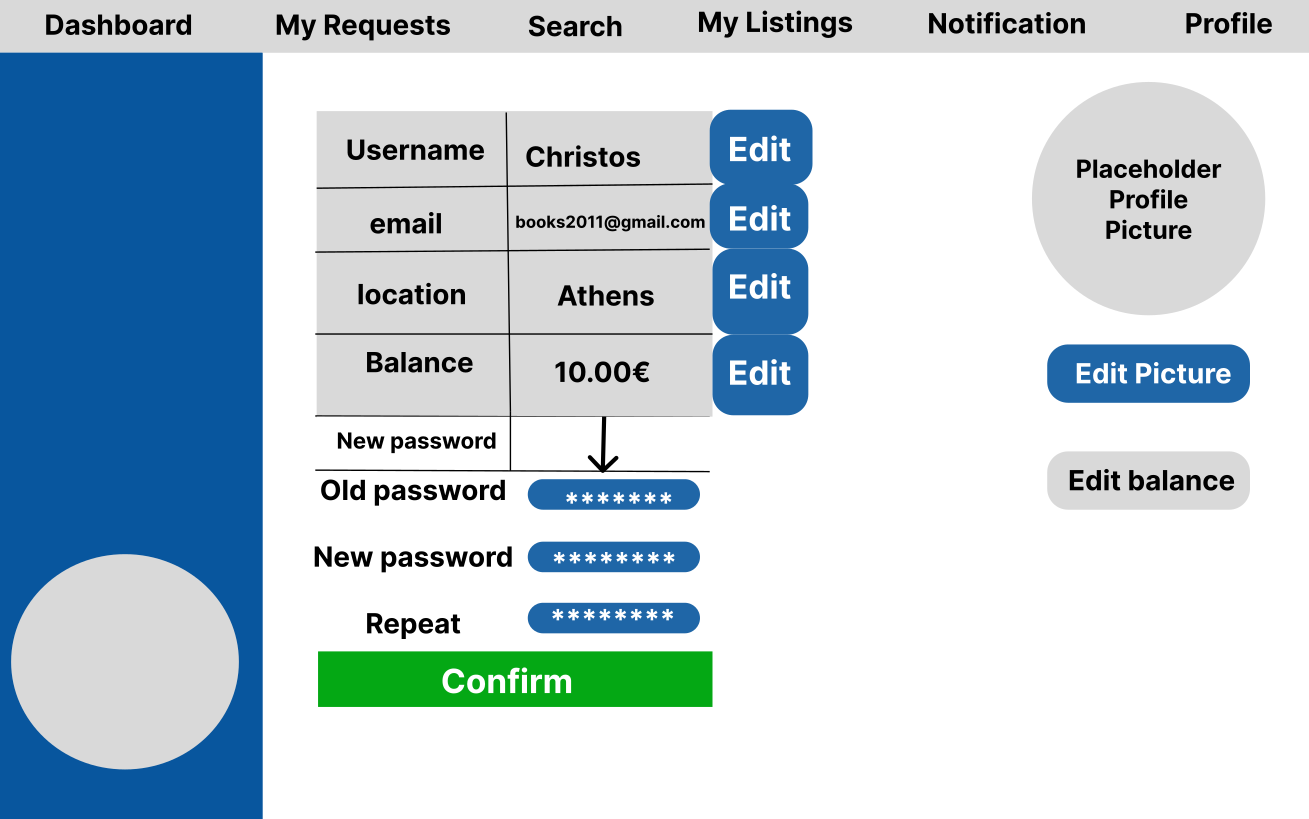
\includegraphics[width=\textwidth]{Mockup Screens/My Profile.png}}
	\caption{Οθόνη "My Profile" λειτουργικότητας}
	\label{Οθόνη "My Profile" λειτουργικότητας}
\end{figure}

Στην οθόνη αυτή υπάρχουν κουμπιά edit δίπλα από κάθε στοιχείο, που θα επιτρέπουν στον χρήστη να κάνει αλλαγές. Επίσης θα μπορεί να αλλάξει τον κωδικό του, όπου θα πρέπει να εισάγει πρώτα τον παλιό του κωδικό, και μετά δύο φορές τον νέο πριν επιβεβαιώσει την αλλαγή. 

Με το κουμπί "Manage" δίπλα στο "Balance" εμφανίζεται επίσης ένα pop up όπου ο χρήστης έχει την επιλογή να προσθέσει ή να αφαιρέσει λεφτά στον/από τον λογαριασμό του. Η οθόνη αυτή φαίνεται στο σχήμα \ref{Οθόνη "Balance" λειτουργικότητας}.

\begin{figure}[H]
    \makebox[\textwidth]{\fbox{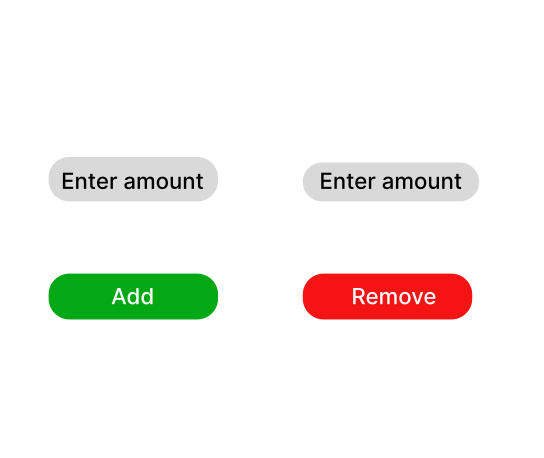
\includegraphics[width=\textwidth]{Mockup Screens/Balance.png}}}
	\caption{Οθόνη "Balance" λειτουργικότητας}
	\label{Οθόνη "Balance" λειτουργικότητας}
\end{figure}

\section{Συμμετοχή και Ρόλοι στη Συγγραφή του Κειμένου}

\begin{enumerate}
	\item \textbf{Γρηγόρης Καπαδούκας:} Author
	\item \textbf{Χρήστος Μπεστητζάνος:} Editor, Contributor
	\item \textbf{Νικόλαος Αυγέρης:} Peer Reviewer
	\item \textbf{Περικλής Κοροντζής:} Peer Reviewer
\end{enumerate}

\section{Αλλαγές από έκδοση σε έκδοση}

\subsection{Από έκδοση v0.1 σε έκδοση v0.2}
\begin{itemize}
    \item Αναδόμηση του κειμένου της περιγραφής ώστε να είναι χωρισμένο σε τμήματα και πιο ευανάγνωστο. 
    \item Προσθήκη του συστήματος των ειδοποιήσεων.
    \item Προσθήκη παραπάνω διευκρινήσεων σχετικά με τη λειτουργικότητα των αιτήσεων και των αναζητήσεων.
    \item Ανανέωση όλων των mock-up screens.
\end{itemize}

\end{document}
